\documentclass{beamer}
\usetheme[pageofpages=of,% String used between the current page and the
                         % total page count.
          bullet=circle,% Use circles instead of squares for bullets.
          titleline=true,% Show a line below the frame title.
          alternativetitlepage=true,% Use the fancy title page.
       %   titlepagelogo=logo-polito,% Logo for the first page.
       %   watermark=watermark-polito,% Watermark used in every page.
       %   watermarkheight=100px,% Height of the watermark.
       %   watermarkheightmult=4,% The watermark image is 4 times bigger
                                % than watermarkheight.
          ]{Torino}

\setbeamertemplate{footline}{
  \begin{beamercolorbox}[wd=\paperwidth,ht=1ex,dp=1ex]{footline}
    \vspace{5pt} \hspace{1em} \insertframenumber/\inserttotalframenumber
  \end{beamercolorbox}
}

\author{Brendon J. Brewer}
\title{STATS 331 -- Introduction to Bayesian Statistics}
\institute{The University of Auckland}
\date{}


\linespread{1.3}
\usepackage{minted}
\usepackage[utf8]{inputenc}
\usepackage{dsfont}
\newcommand{\given}{\,|\,}


\begin{document}

\frame{\titlepage}

\begin{frame}
\begin{center}
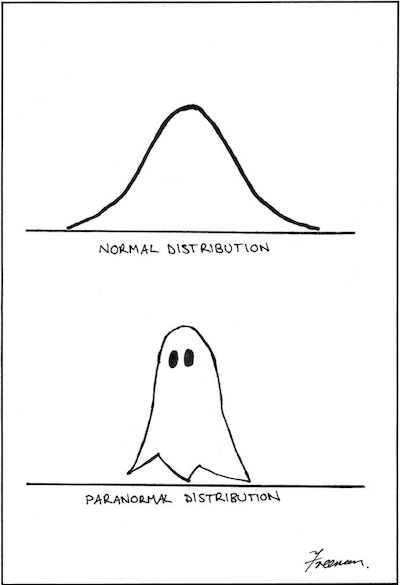
\includegraphics[width=0.4\textwidth]{images/paranormal.png}

Credit: Matthew Freeman
\end{center}

\end{frame}



\begin{frame}
\centering
\large
Heavy-Tailed Models and Multiple Regression

\end{frame}


\begin{frame}
\frametitle{Fake Data with Outlier}
I generated some data from $y=x$ with $\sigma=3$, then manually added two
extreme outliers:

\begin{center}
\includegraphics[width=0.6\textwidth]{images/outlier_data.pdf}
\end{center}

\end{frame}

\begin{frame}
\frametitle{Fake Data with Outlier}
\begin{itemize}
\item What will happen if we run the linear regression model, as it is, on this
data? \pause
\item The classical least squares estimate would be dragged substantially towards
the outliers (by reducing the slope).\pause
\item With the current model, the same thing will happen in the Bayesian framework,
because of the choice of sampling distribution/likelihood --- particularly,
the light tails of the gaussian.
\end{itemize}
\end{frame}

\begin{frame}
\frametitle{Running the Model}
Let's run the regression model on this data, and see what the posterior
distributions look like, and whether they accurately recover
$y=x$ and $\sigma=1$.\pause

Surprisingly, the posterior distributions for $\beta_0$ and $\beta_1$ aren't
actually that bad, but the uncertainties get inflated because $\sigma$ has
to be super high to explain the outliers.
\end{frame}


\begin{frame}
\frametitle{Conclusion}
The best way of explaining this data, with the current model, is if $\sigma$
is much larger than 1 and the slope $\beta_1$ is less than 1.
{\bf If we believe the model assumptions}, this is the
answer, and that's that.\pause

However, often model assumptions aren't truly reliable but are chosen out of
tradition or habit. We are free to change the model to one that
{\bf expects} the odd outlier.
\end{frame}


\begin{frame}
\frametitle{Student-$t$ Distributions from Wikipedia}

\begin{center}
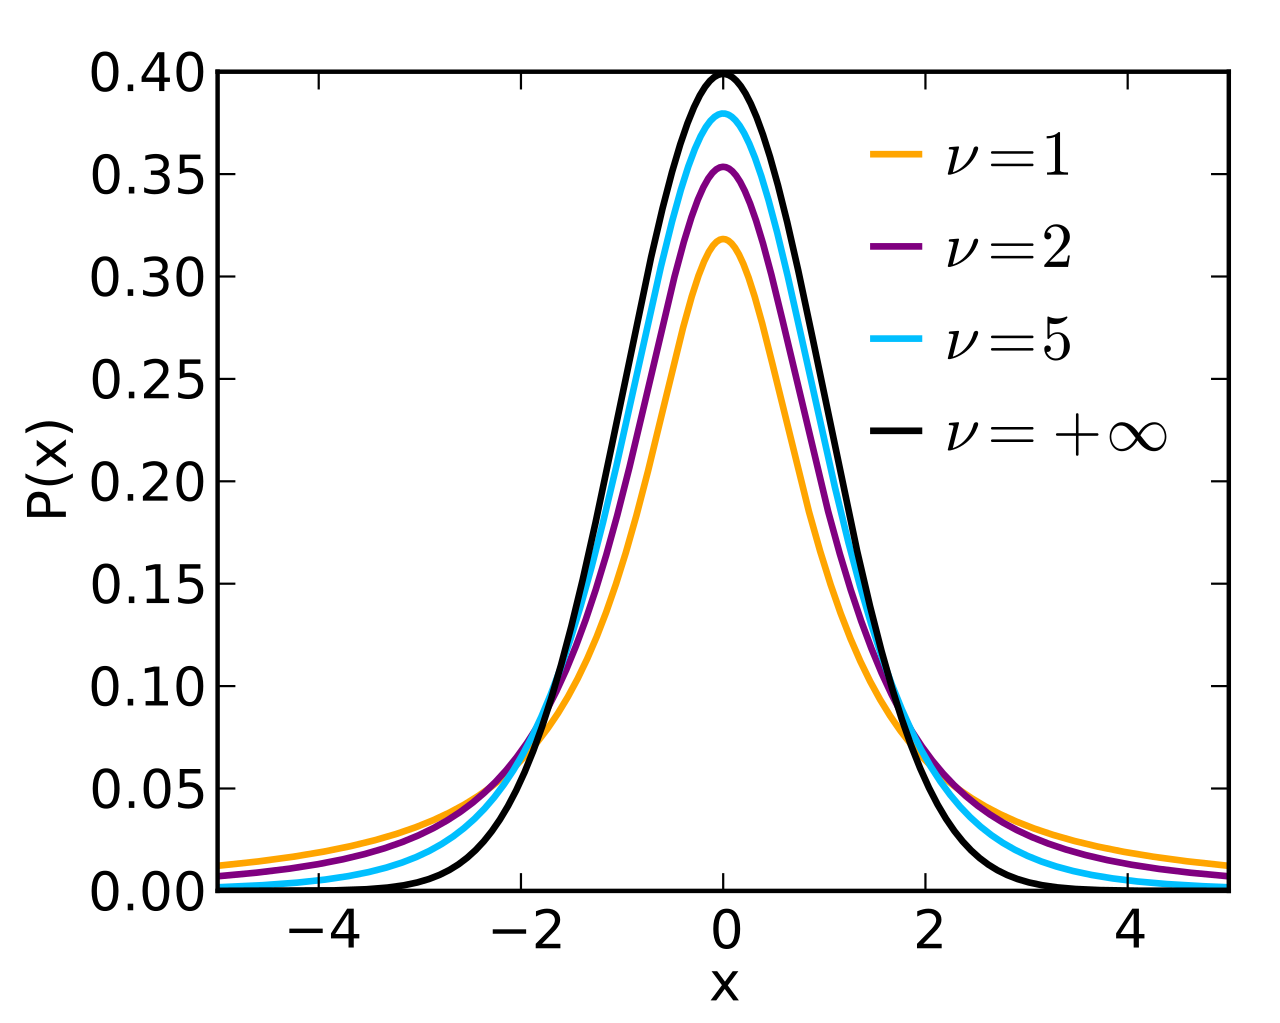
\includegraphics[width=0.7\textwidth]{images/t_distribution.png}
\end{center}
\end{frame}

\begin{frame}[fragile]
\frametitle{Student-$t$ Distributions in JAGS}
We will use the Student-$t$ distribution as a drop-in replacement for the
normal distribution in our model. We simply replace
\begin{minted}{r}
dnorm(mu, 1/sigma^2)
\end{minted}
with
\begin{minted}{r}
dt(mu, 1/sigma^2, nu)
\end{minted}
\pause
{\bf Note}: The extra parameter \mintinline{r}{nu}, which controls the
tail behaviour, will need a prior (low $\nu$ = heavy tails,
high $\nu$ = approximately normal).
\end{frame}

\begin{frame}[fragile]
\frametitle{Modified Parts of the Regression Model}
\footnotesize
\begin{minted}{r}
log_nu ~ dunif(-2, 5)
nu <- exp(log_nu)

for(i in 1:length(y))
{
    y[i] ~ dt(beta0 + beta1*(x[i] - mean(x)), 1/sigma^2, nu)
}
\end{minted}
\pause

{\bf Note}: \mintinline{r}{sigma} is no longer a standard deviation, but is still
a scale parameter (controls width).

\end{frame}


\begin{frame}[fragile]
\frametitle{Results from Heavy-Tailed Model}
The results from the heavy tailed model are a fair bit better,
and $\sigma$ (even though it has changed its interpretation a bit)
is much smaller. It can explain the outliers by having a low value
of $\nu$ instead.\\[0.5em]\pause

We can look at the posterior for $\log(\nu)$ (which had a uniform prior)
to see, whether large values (i.e., approximately gaussian shape) are ruled out.

\end{frame}

\begin{frame}[fragile]
\frametitle{One Parameter Space}
Instead of doing model selection to test the
normal model against the Student-$t$
(which we cannot do here as MCMC does not
calculate marginal likelihoods), we can sometimes create something like
the two models in the one parameter space, and just do parameter estimation.
This is a good strategy in general.

\end{frame}


\begin{frame}
\frametitle{Conclusion About Outliers}

{\em
``Sometimes outliers are bad data, and should be excluded,
such as typos. Sometimes they are Wayne Gretzky or
Michael Jordan, and should be kept.''}

- Neil McGuigan, on stackexchange.com\\[1em]

\pause

One size does not fit all --- whether outliers should have a big effect
or not depends on your prior information.

\end{frame}

\begin{frame}

\Large
\begin{center}
Multiple Linear Regression
\end{center}

\end{frame}



\begin{frame}
\frametitle{Multiple Linear Regression}
\begin{itemize}
\item We will now look at some examples of multiple linear regression.\pause
\item This is a relatively straightforward extension of simple linear
regression, but we just have more than one explanatory variable.\pause
\item There are whole courses about these kinds of models (e.g., STATS 330)
but they are usually from a classical/frequentist viewpoint.
\end{itemize}
\end{frame}



\begin{frame}
\frametitle{Clocks Data}
How does the age of a grandfather clock, and the number of bidders,
affect the price it sells for at an auction?

\begin{center}
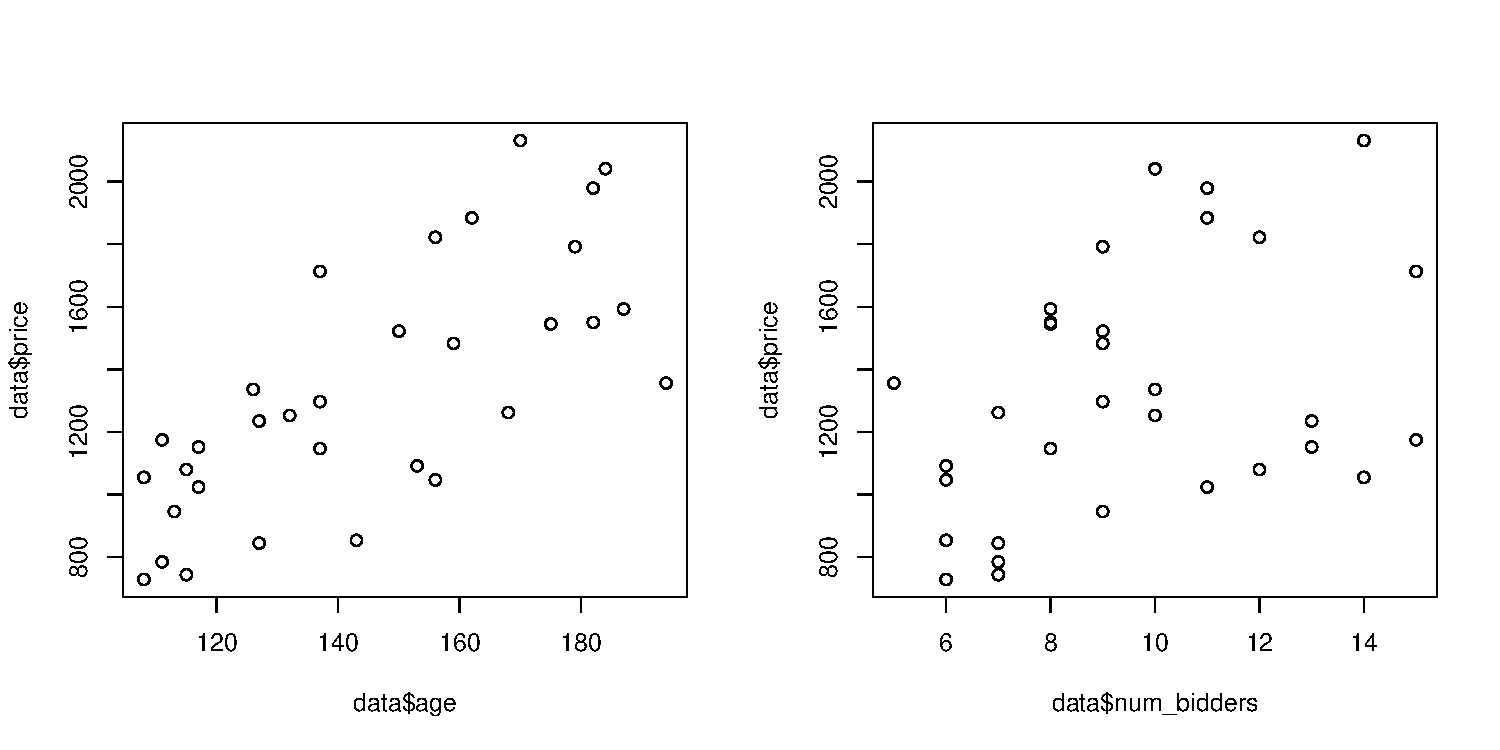
\includegraphics[width=0.8\textwidth]{images/clocks.pdf}
\end{center}

\end{frame}


\begin{frame}
\frametitle{Multiple Regression Assumptions}
We just need to add extra terms to the regression assumptions.

\begin{align}
y_i &= \beta_0 + \beta_1 x_{i, 1} + \beta_2 x_{i, 2} + \epsilon_i \\
\epsilon_i &\sim \textnormal{Normal}(0, \sigma^2)
\end{align}

\pause

However, when we implement this in JAGS, we will (a) center the
explanatory variables, (b) rename the nodes in the JAGS code
so they match the names in the data, and (c) use the wide
normal priors for coefficients --- for no reason really.

\end{frame}


\begin{frame}[fragile]
\frametitle{JAGS Code for Clocks}
\tiny

\begin{minted}{r}
model
{
    beta0 ~ dnorm(0, 1/1000^2)
    beta1 ~ dnorm(0, 1/1000^2)
    beta2 ~ dnorm(0, 1/1000^2)
    log_sigma ~ dunif(-10, 10) # Log-uniform prior for sigma
    sigma <- exp(log_sigma)

    for(i in 1:N)
    {
        price[i] ~ dnorm(beta0
                            + beta1*(age[i] - mean(age))
                            + beta2*(num_bidders[i] - mean(num_bidders)),
                         1/sigma^2)
    }
}
\end{minted}

\end{frame}


\begin{frame}[fragile]
\frametitle{Clocks Results}
Let's run the MCMC. We should see that the coefficients are both
almost certainly positive.

\end{frame}


\begin{frame}[fragile]
\frametitle{Interaction Term}
We can look for curvature/nonlinearity in the regression relationship,
so we are fitting a curved surface rather than a plane.
\tiny
\begin{minted}{r}
model
{
    # Repeat same priors here...

    # Extra parameter
    beta3 ~ dnorm(0, 1/1000^2)
    for(i in 1:N)
    {
        price[i] ~ dnorm(beta0
                            + beta1*(age[i] - mean(age))
                            + beta2*(num_bidders[i] - mean(num_bidders))
                            + beta3*(age[i] - mean(age))*
                                    (num_bidders[i] - mean(num_bidders)),
                         1/sigma^2)
    }
}
\end{minted}

\end{frame}


\begin{frame}[fragile]
\frametitle{Clocks Results}
Assuming there is an interaction term, it is also positive.

\end{frame}



\begin{frame}[fragile]
\frametitle{Can We Do Model Selection?}
Statisticians often have the instinct to do ``model selection'' (in the case
of regression it is also called ``variable selection'') to see which terms
should be included. We could have something like this:
\begin{align}
H_0:\quad& \beta_3 = 0 \\
H_1:\quad& \beta_3 \neq 0.
\end{align}
\pause
However, this would require either marginal likelihoods (which JAGS cannot
compute) or a spike-and-slab prior (which it can do with hacks --- we'll
see this in the $t$-test lectures).
\end{frame}

\begin{frame}
\frametitle{Warning About Priors}
\begin{itemize}
\item If the number of explanatory variables is large, you need a prior
for a large number of coefficients.\pause
\item Vague priors can become more dodgy as the number of
parameters increases!.\pause
\item ``Hierarchical models'' often needed --- quite tricky to use in
regression models.
\end{itemize}

\end{frame}


\begin{frame}
\frametitle{Catheter Data}
Here's another multiple regression dataset.
The response variable is the length of a catheter needed for a medical procedure.
The height and weight of the patient are the explanatory variables.
You would expect a longer catheter is needed as height and weight increases
--- but height and weight are also strongly correlated with each other.

\end{frame}

\begin{frame}
\frametitle{Catheter Data}
This plot shows the correlation between the explanatory variables
(the response variable is not shown).

\begin{center}
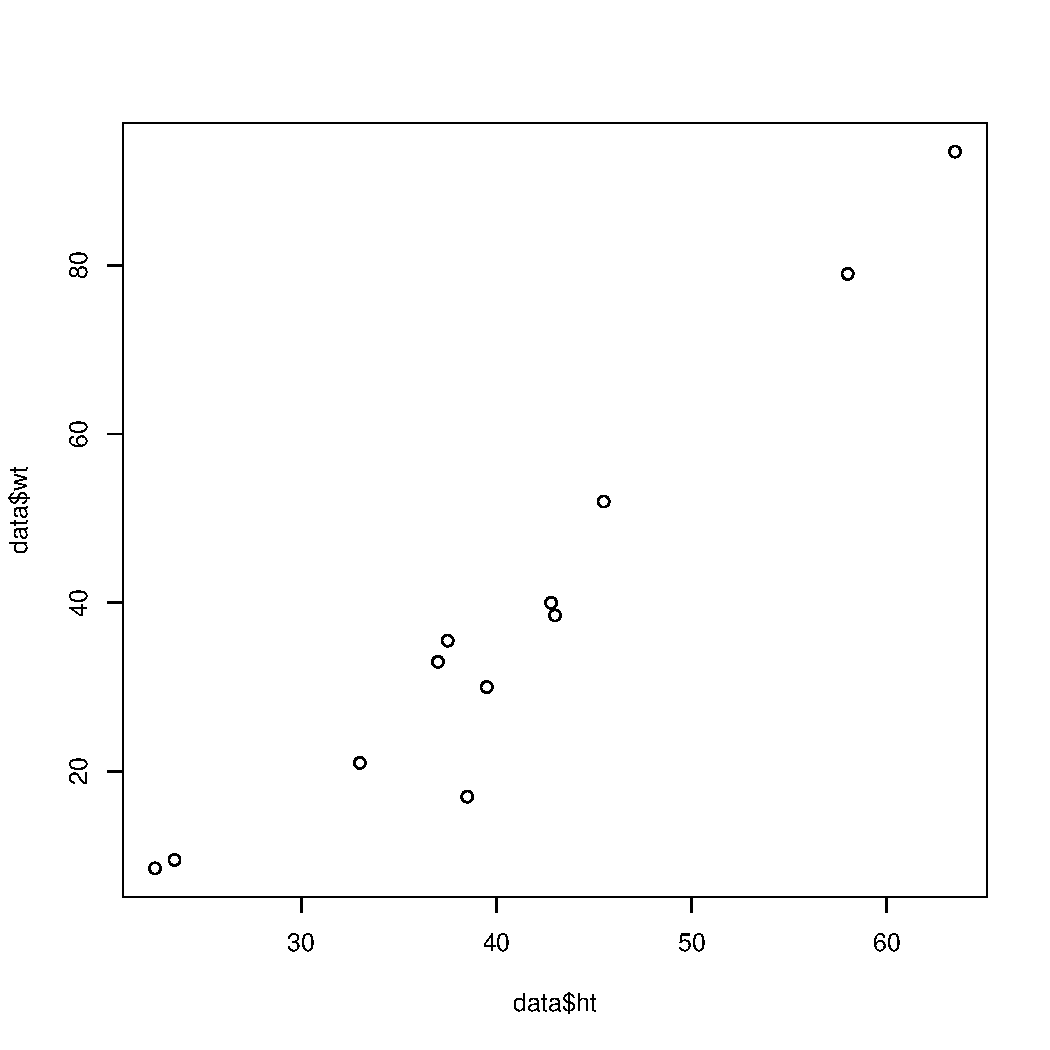
\includegraphics[width=0.4\textwidth]{images/catheter.pdf}
\end{center}

\end{frame}


\begin{frame}
\frametitle{Catheter Posterior}
Let $\beta_1$ be the coefficient for height and $\beta_2$ the coefficient
for weight:
\begin{center}
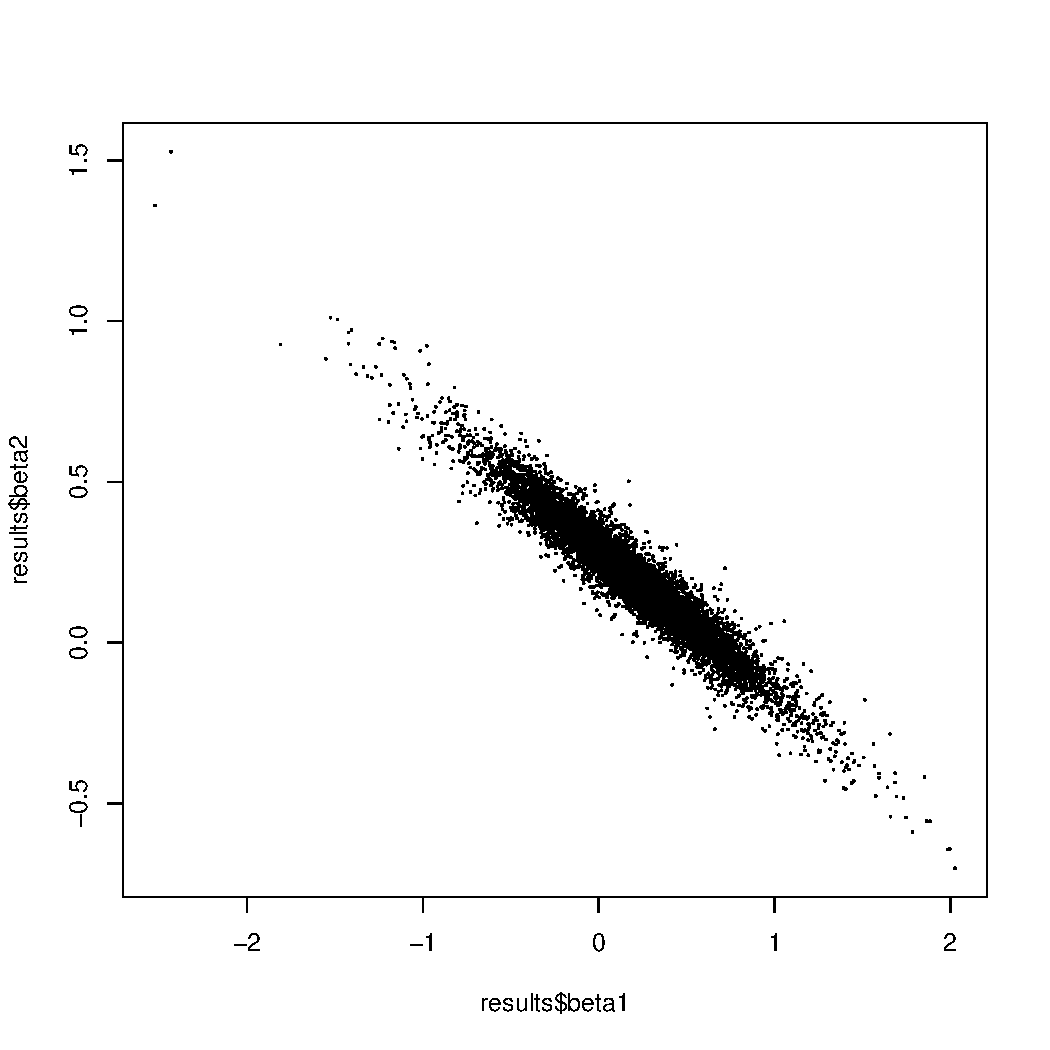
\includegraphics[width=0.4\textwidth]{images/catheter_posterior.pdf}
\end{center}
We don't have to do anything about the correlation between
the explanatory variables. Its consequences appear in the results.

\end{frame}


\begin{frame}
\frametitle{Linear Regression Conclusions}
\begin{itemize}
\item This is one situation where the classical and Bayesian results are
numerically similar (if the Bayesian uses wide priors). We just get the
improved interpretation of the posterior distribution and its summaries.\pause
\item One other benefit of our approach is that it is easy to modify the
assumptions if necessary (for example, our use of the $t$-distribution).
If you are just using \mintinline{r}{lm()} you
are stuck with standard assumptions.
\end{itemize}

\end{frame}


\end{document}

